\subsection{Funktionsweise vom AES Algorithmus}
\label{sec:aes}
\setlength{\parindent}{0pt}

Advanced Encryption Standard (AES) ist ein symmetrischer Blockchiffre Algorithmus zur 
Verschlüsselung sensibler Daten wie VPN Verbindungen, HTTPS Anfragen 
(siehe Abbildung~\ref{fig:http_verbindungsaufbau}) und WLAN (WPA2). 
Entwickelt wurde er 2001 vom NIST. AES arbeitet mit Schlüssellängen von 128, 192 oder 256 Bit, 
wobei längere Schlüssel sicherer sind. Die Blockgröße beträgt stets 128 Bit, da AES eine Blockchiffre 
ist. Die Anzahl der Runden hängt von der Schlüssellänge ab: 
\begin{itemize}
    \item 128 Bit: 10 Runden
    \item 192 Bit: 12 Runden
    \item 256 Bit: 14 Runden
\end{itemize}
Der AES-Schlüssel kann beliebig gewählt werden, muss jedoch sicher erzeugt und geheim gehalten werden, um 
die Integrität des Verfahrens zu gewährleisten. Häufig wird der Schlüssel durch kryptographische Verfahren 
wie das Password-Based Encryption (PBE) oder durch den Einsatz eines sicheren Schlüsselaustauschverfahrens 
wie Diffie-Hellman bestimmt. Der AES-Algorithmus selbst unterstützt keine eigene Schlüsselverteilung, sondern 
nutzt stattdessen den vom Anwender oder einem sicheren Protokoll bereitgestellten Schlüssel.


Jeder 128-Bit-Block wird als 4$\times$4-Matrix dargestellt:
\[
\begin{bmatrix}
c_0  & c_1  & c_2  & c_3 \\
c_4  & c_5  & c_6  & c_7 \\
c_8  & c_9  & c_{10} & c_{11} \\
c_{12}  & c_{13}  & c_{14} & c_{15}
\end{bmatrix}
\]

Wie in Abbildung~\ref{fig:qualen_AES} dargestellt, umfasst jede Runde die Schritte \textit{SubBytes}, \textit{ShiftRows}, \textit{MixColumns} und \textit{Add Round Key}. 
In der letzten Runde wird \textit{MixColumns} über\-sprungen \cite{AES_Algorithmus_2} \cite{AES_Algorithmus_3} \cite{AES_Algorithmus} \cite{Blockchiffre}.

\begin{figure}[H]
	\centering
	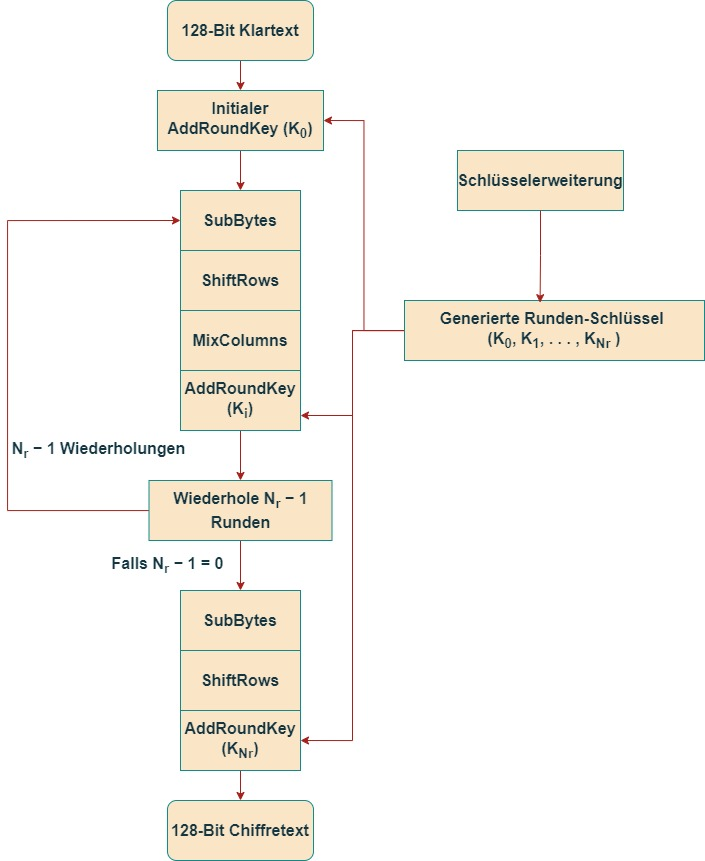
\includegraphics[width=0.45\textwidth]{sections/matheo/final.jpg}
	\caption{AES Ablauf}
	\label{fig:qualen_AES}
\end{figure}



\subsubsection{S-Box}
Die S-Box (Substitution-Box) dient zur nichtlinearen Byte-Substitution, um die Beziehung zwischen Schlüssel und Chiffretext zu verschleiern. Jedes Eingangsbyte \(b\) (außer 0) wird im Galois-Feld \(GF(2^8)\) inversiert:
\[
b' = b^{-1} \mod (x^8 + x^4 + x^3 + x + 1)
\]
Dabei ist \(x^8 + x^4 + x^3 + x + 1\) das standardmäßige irreduzible Polynom. Das Ergebnis wird durch eine lineare Transformation angepasst:
\[
s_i = A \cdot b_i + c
\]
wobei \(A\) eine $8 \times 8$-Matrix ist und \(c\) eine Konstante \cite{Endliche_körper} \cite{S_Box}.

\subsubsection{round key}

Der 128-Bit-Schlüssel wird in vier 32-Bit-Wörter $w[0], w[1], w[2], w[3]$ unterteilt. 
Der Wert $g(w[3])$ wird durch eine zyklische Linksverschiebung von $w[3]$ berechnet, 
gefolgt von einer Byte-Substitution jedes Bytes mittels der S-Box. Anschließend wird 
der Rundenkonstantenwert $R_1$ hinzugefügt:
\[
g(w[3]) = \text{Substitute}(\text{Shift}(w[3])) \oplus R_1
\]
Die weiteren Wörter werden durch XOR ($\oplus$) der entsprechenden vorherigen Werte berechnet:
\begin{align*}
w[4] &= w[0] \oplus g(w[3]), \\
w[5] &= w[4] \oplus w[1], \\
w[6] &= w[5] \oplus w[2], \\
w[7] &= w[6] \oplus w[3]
\end{align*}
Der erste Rundenschlüssel ergibt sich schließlich durch Kombination der Wörter $w[4], w[5], w[6], w[7]$:
\[
\text{Rundenschlüssel}_1 = w[4], w[5], w[6], w[7]
\]

\subsubsection{SubBytes}
\textit{SubBytes} ersetzt jedes Byte des Datenblocks durch den entsprechenden Wert aus der S-Box, wobei die Bytewerte als Adressen dienen. Zum Beispiel:
\begin{table}[H]
    \resizebox{0.3\textwidth}{!}{
    \begin{tabular}{|c|cccccccccc|}
    \hline
       & \dots & X4 & X5 & X6 & X7 & X8 & X9 & XA & XB & \dots \\
    \hline
    0X & \dots & 63 & 7C & 77 & 7B & F2 & 6B & 6F & C5 & \dots \\
    1X & \dots & 30 & 01 & 67 & 2B & FE & D7 & AB & 76 & \dots \\
    2X & \dots & CA & 82 & C9 & 7D & FA & 59 & 47 & F0 & \dots \\
    3X & \dots & AD & D4 & A2 & AF & 9C & A8 & 51 & A3 & \dots \\
    4X & \dots & 40 & 8F & 92 & 9D & 38 & F5 & BC & B6 & \dots \\
    5X & \dots & DA & 21 & 10 & FF & F3 & D2 & CD & 0C & \dots \\
    6X & \dots & 13 & EC & 5F & 97 & 44 & 17 & C4 & A5 & \dots \\
    7X & \dots & 33 & 85 & 45 & F9 & 02 & 7F & 50 & 3C & \dots \\
    \dots & \dots & \dots & \dots & \dots & \dots & \dots & \dots & \dots & \dots & \dots \\
    \hline
    \end{tabular}
    }
    \caption{Ausschnitt einer S-Box im AES-Algorithmus \\ („X“ ist ein Platzhalter)}
\end{table}



\subsubsection{ShiftRows}
\textit{ShiftRows} verschiebt die Reihen der 4 x 4-Matrix zyklisch: Die $n$-te Reihe wird um $(n-1)$ Stellen nach links verschoben. Zum Beispiel:
\[
\begin{bmatrix}
c_0  & c_1  & c_2  & c_3  \\
c_4  & c_5  & c_6  & c_7  \\
c_8  & c_9  & c_{10} & c_{11} \\
c_{12} & c_{13} & c_{14} & c_{15}
\end{bmatrix}
\quad\rightarrow\quad
\begin{bmatrix}
c_0  & c_1  & c_2  & c_3  \\
c_5  & c_6  & c_7  & c_4  \\
c_{10} & c_{11} & c_8  & c_9  \\
c_{15} & c_{12} & c_{13} & c_{14}
\end{bmatrix}
\]

\subsubsection{MixColumns}
MixColumns sorgt für eine Mischung der Spalten, indem jede Spalte der Matrix als Polynom im Galois-Feld 
\(GF(2^8)\) betrachtet wird. Jede Spalte wird mit einem festen Polynom \(a(x) = 03x^3 + 01x^2 + 01x + 02\) 
multipliziert, wobei die Multiplikation modulo \(x^4 + 1\) erfolgt. Dieser Schritt verteilt die Bits der Eingabe, 
um eine stärkere Diffusion zu gewährleisten.

\subsubsection{Add Round Key}
In Add Round Key wird jede Byte-Position des Blocks mit dem entsprechenden Byte des Rundenschlüssels 
XOR-verknüpft. Dieser Schritt sorgt dafür, dass der Hauptschlüssel in jede Runde einfließt.

\subsubsection{Sicherheit gegenüber Quantenangriffen}
Ein wesentlicher Vorteil von AES im Vergleich zu anderen Algorithmen, wie etwa RSA, ist seine Sicherheit 
gegen theoretische Angriffe von Quantencomputern. Quantenalgorithmen wie Shor's Algorithmus sind in der Lage, 
die Primfaktorzerlegung und das Diskrete Logarithmusproblem effizient zu lösen, was RSA und ähnliche Verfahren anfällig 
für Angriffe macht. Im Gegensatz dazu beruht AES nicht auf der Schwierigkeit der Faktorisierung von Primzahlen, sondern 
auf der sogenannten \textit{Diffusion} und \textit{Verkettung} der Daten, die von Quantencomputern nicht so leicht durchbrochen 
werden können. Daher gilt AES auch in einer Ära der Quantencomputer als sicher, solange die Schlüssel ausreichend lang sind.
